Tässä luvussa on käyty jokainen harjoitustyö läpi omassa alaluvussaan.
Harjoitukset voivat olla mahdollisesti jatkoa edelliseen, mutta ovat
silti selkeyden vuoksi esitelty erillisillä kappaleilla.

Luvun lopusta löytyy Tuntikirjanpito harjoitustehtäviin käytetystä ajasta.

\section{Harjoitus 2}

Versionhallinnan käyttö on tullut aloitettua lähes 10 vuotta sitten ja on
välttämätön työkalua niin töissä, opiskelussa kuin vapaa-ajan projekteissakin,
joten uskon käytön vähintään peruskäytön hallitsevan. Tämän vuoksi erillistä
harjoitus ohjeen mukaista harjoitus2\_vastaus.txt-tiedostoa ei ole lisätty.

Käytössä on lisäksi ssh-avaimet, kuten harjoituksessa viitattiin. Näiden
lisäksi myös commitit allekirjoitetaan ja käytössä submoduuleja. Näistä oli
tarkemmin selitystä aloitus-osiossa.

Oppimispäiväkirja on myös versionhallinnassa ja PDF-muoto siitä generoidaankin
automaattisesti Github Actioneilla, jotka ovat merkittävä apu asioiden
automatisoinnissa kätevästi versionhallinnan kanssa.

\section{Harjoitus 3}

Android Studion asentamisesa on kerrottu tarkemmin aloitus-osiossa.

Oppimispäiväkirja-repository ja sen myötä myös harjoituksien kansiot
sijaisevat WSL:n tiedostojärjestelmässä. Tähän on keino päästä käsiksi kuten
mm. verkkojakoihin, toisiin kovalevyihin yms. Android Studio ei kuitenkaan
toimi tämän kautta vaan näyttää \ref{fig:android-studio-path-not-writable}
mukaisen virheen, ettei kansio ole kirjoitusoikeuksia.

\begin{figure}[h!]
    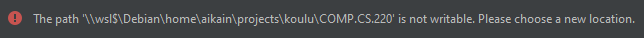
\includegraphics[width=\textwidth]{figures/android-studio-path-not-writable.png}
    \caption{Kuvankaappaus Android Studio virheestä kirjoittaa kansioon}
    \label{fig:android-studio-path-not-writable}
\end{figure}

Projektin voi kuitenkin luoda muutoin WSL:n puolelle ja sen jälkeen avata
Android Studiolla. Tästä kuitenkin aiheutuu uusi ongelma; Gradle ei saa
syncattua haluamiaan asioita vaan sanoo ''virhe, yritä uudelleen'' tarkentamatta
mikä virhe. Logeista löytyy hiukan tarkempi virhe:

\begin{displayquote}
GradleConnectionException: Operation result has not been received
\end{displayquote}

Tämän virheen perusteella ei kuitenkaan löydy mitään Android Studioon itseensä
liittyvää vaan kaikki viittaavat kahteen Intellij IDEAn issueeseen (joka toki
tässä tapauksessa on tarpeeksi lähellä), mutta molemmissa puhutaan Android-
lisäosan kytkemisestä pois päältä ja se ei oikein toimi ratkaisuna tähän
tilanteeseen.

On hyvin mahdollista, että virhe johtuu SDK:n sijaitsemisesta Windowsin
puolella kun kaikki muut (projekti, gradle, jdk) sijaisevat WSL:n sisällä.
Kuitenkin kokemuksen pohjalta yleensä fyysisten laitteiden kanssa kommunikointi
WSL:n sisältä käsin on hyvin nihkeää ja jo emulaattorinkin käyttö saattaisi
tuottaa ongelmia, joten ei ole mielekästä lähteä asentamaan Android SDK:ta ja
kaikkea siihen liittyvää WSL:n sisälle.

Pitkälti siis ainut toimiva ja aikaa säästävä ratkaisu on pitää projektit
Windowsin puolella. Kuitenkaan yksittäisten projektin vuoksi en ole siirtämässä
versionhallintaa ja kaikkea muuta configuraatiota toimimaan WSL:n ulkopuolella,
joten tarvitaan keino pitää repo WSL:ssä, mutta harjoitustehtävät Windowsin
puolella. Ensimmäisenä tähän tulee mielenä yksinkertaisesti käyttää symboolista
linkkiä.

\begin{lstlisting}[
    basicstyle=\small,
    label={lst:symbolic-link-harjoitustehtavat},
    language=bash,
]
    # ln -s /mnt/c/Users/Aikain/AndroidStudioProjects/mobiiliohjelmointi-kurssi-harjoitustehtavat/ harjoitustehtavat
\end{lstlisting}

Symboolin linkki näkyy kuitenkin Gitille symboolisena linkkinä eikä normaaleina
tiedostoina, mikä toki on täysin perusteltua mm. tietoturvasyistä. Puolestaan
ns. kovan linkin tekeminen ei ole mahdollista kansioille. Vaihtoehtoisesti
voisi kokeilla linkin tekemistä toisinpäin
\parencite{StackoverflowWSLSymlink}.

\begin{lstlisting}[
    basicstyle=\small,
    label={lst:powershell-link-harjoitustehtavat},
    language=PowerShell,
]
    New-Item -ItemType SymbolicLink -Path ''C:\Aikain\Users\AndroidStudioProjects\mobiiliohjelmointi-harjoitustehtavat'' -Target ''\\wsl$\Debian\home\aikain\projects\COMP.CS.220\harjoitustehtavat''
\end{lstlisting}

Tämä kuitenkin aiheuttaa jälleen samat ongelmat kuin aiemmin Android Studion
kanssa kun yritti käyttää suoraan WSL:n sisällä olevaa sijaintia.

Ei ehkä niin hyvänä ratkaisuna, mutta kuitenkin toistaiseksi toimiva ratkaisu
saadaan käyttämällä bind mountia \parencite{BaeldungBindMounts}.

\begin{lstlisting}[
    basicstyle=\small,
    label={lst:bind-mount-harjoitustehtavat},
    language=bash,
]
    $ mount -o bind /mnt/c/Users/Aikain/AndroidStudioProjects/mobiiliohjelmointi-harjoitustehtavat /home/aikain/projects/koulu/COMP.CS.220/harjoitustehtavat
\end{lstlisting}

Versionhallintaan lisätessä kiinnitin huomiota tarkemmin noihin gradle
tiedostoihin. Jotenkin olen sitä vastaan, että jar-tiedoston laittaisi
versionhallintaan, mutta Gradlen dokumentaatiossa
\parencite{GradleDocsGradleWrapper} sanotaan seuraavasti:

\begin{displayquote}
To make the Wrapper files available to other developers and execution
environments you’ll need to check them into version control. All Wrapper files
including the JAR file are very small in size. Adding the JAR file to version
control is expected. Some organizations do not allow projects to submit binary
files to version control. At the moment there are no alternative options to the
approach.
\end{displayquote}

Toistaiseksi siis laittelen nämä versionhallintaan, mutta olisi hyvä jos tähän
olisi parempi ratkaisu.

Lisäksi .idea-kansion sisältö ei ole oletuksena kokonaan .gitignore:ssa.
Ilmeisesti toki pääosa käyttäjistä käyttää Android Studio:ta, mutta silti IDEn
configuraation laittaminen versionhallintaan ei tunnu oikealta ratkaisulta,
varsinkin kun Android Studio osaa avata projektin ilman niitä ja mitään
projektille merkittäviä asioita ei pitäisi olla IDEn configuraatiossa, jotta
muunmuassa CI/CD toimii ongelmitta kun lähtökohtaisesti ne eivät ole tietoisia
IDEn confeista.

\section{Harjoitus 4}

Tarkoitus painottaa Kotlinilla tekemistä ja tehdä varsinkin projekti
Kotlinilla, joten tässäkin valittu pienempi eli harjoitus 4 javalla tehtäväksi
ja suurempi eli harjoitus 5 Kotlinilla tehtäväksi.

Painotus opiskelussa on ollut Composessa, jota puolestaan ei voi käyttää Javan
kanssa \parencite{StackoverflowComposeInJava}, joten alkuun pääseminen vaatii
muutaman minuutin mietintä tauon, mutta onneksi Android Studio alustaa
valmiiksi uuden projektin luonnin yhteydessä tarvittavat asiat.

\begin{wrapfigure}{r}{0.4\textwidth}
    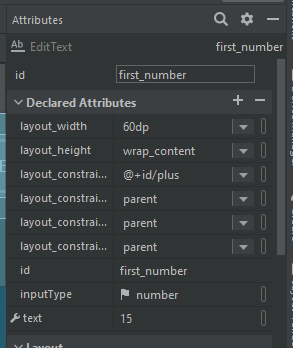
\includegraphics[width=0.4\textwidth]{figures/exercise-4-attributes.png}
    \caption{Kuvankaappaus Android Studio Design-työkalun attribuuteista}
    \label{fig:exercise-4-attributes}
\end{wrapfigure}

Design-työkalun avulla saa lisättyä helposti tarvittavat osat, mutta jotenkin
graaffisen käyttöliittymän kautta kuvassa \ref{fig:exercise-4-attributes}
näkyvien tietojen täyttäminen ei suju, joten aika vaihtaa Split-tilaan ja
muokata XML:ää suoraan. Tämä sujuukin suoraan helpommin ja jopa yleensä
päänvaivaa aiheuttavat app:layout\_constraintX\_toXOf -asetukset menevät
sujuvasti tällä kertaa.

Aluksi lisään kentät suoraan valmiina olevaan ConstraintLayout:in alle, mutta
tästä aiheutuu se etteivät ne ole nätisti tasattuna yhteen riviin vaan
painikkeen ollessa korkeampi on sen keskikohta selvästi alempana kuin muilla.
Tämän voisi sinääli korjata vain nopeasti marginilla, joka tuntuu huonolta
ratkaisulta. Hetken pohdinnan jälkeen saankin laitettua toisen
ConstraintLayout:in, jonka korkeus on vain sisällön verran ja saan sisällön
keskitettyä pystysuunnassa kyseisen komponentin suhteen. Hiukan paddingia
ConstraintLayout:lle ja numerokentille leveydet niin saadaan siististi yhteen
riviin tasaisin välein kuvan \ref{fig:exercise-4-constraint-layout} mukaisesti.

\begin{figure}[h!]
    \centering
    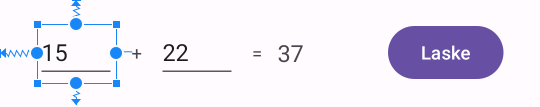
\includegraphics[width=0.8\textwidth]{figures/exercise-4-constraint-layout.png}
    \caption{Kuvankaappaus komponenttien sijoittelusta}
    \label{fig:exercise-4-constraint-layout}
\end{figure}

UI:n tultua valmiiksi viewBinding-ominaisuuden enablointi ja sen jälkeen
saadaankin helposti lisättyä painikkeelle onClickListener, joka ottaa kentistä
luvut ja laskee ne yhteen ja laittaa tulos-kenttään.

\begin{wrapfigure}{rl}{0.3\textwidth}
    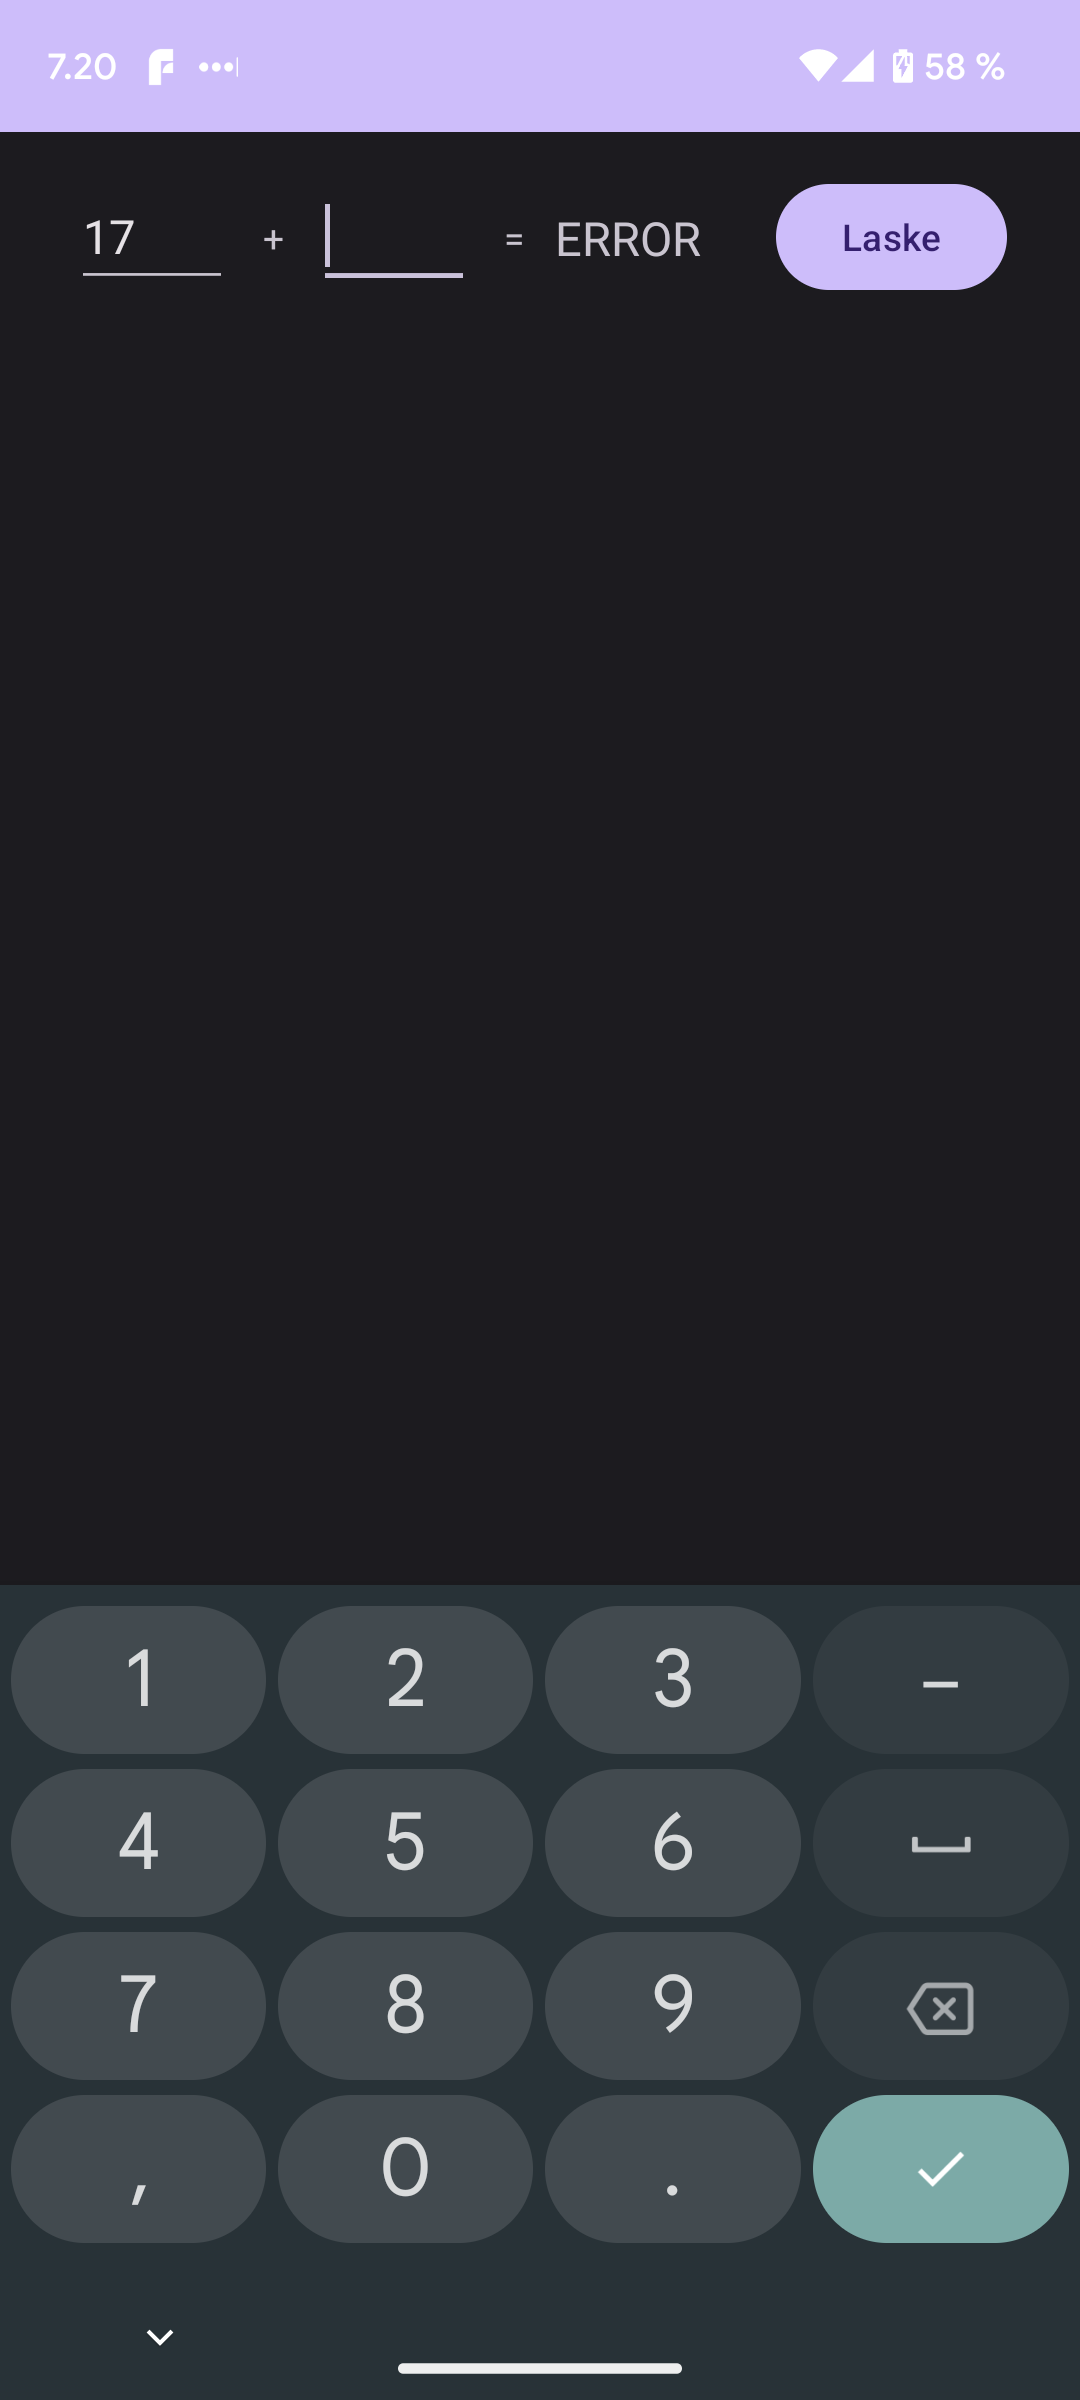
\includegraphics[width=0.3\textwidth]{figures/exercise-4-final.png}
    \caption{Kuvankaappaus lopullisesta sovelluksesta puhelimessa}
    \label{fig:exercise-4-final}
\end{wrapfigure}

Lopulta emulaattorissa toimisen jälkeen vielä hyvä hetki kokeilla, että toimii
sujuvasti puhelimellakin kuten kuvassa \ref{fig:exercise-4-final} näkyy.

Android Studio auttaa vielä nopeasti poistamaan tekstien kovakoodaukset ja
käyttämään strings-resursseja. Parannettavaa näinkin piennessä sovelluksessa
olisi vielä mm. saavutettavuuden suhteen sekä automaattisten testien
tekemisessä. Toki parannettavaa löytyy aina, joten jätetään sovellus tämän
harjoituksen osalta tähän.

\tipbox{
\textbf{Miksi packagen nimen alkuun in.aika?}

Harjoituksissa ja projekteissa esiintyy in.aika-verkkotunnusta. Tämä voi
vaikuttaa hiukan oudolta aluksi, että käytössä Intialainen verkkotunnus. Tähän
on kuitenkin yksinkertainen selitys. Olen pitkään käyttänyt nimimerkkiä
"Aikain" ja kuten jokaisella ''IT-nörtillä'' niin pitäähän minullakin olla
omaverkkotunnus (tai tänä päivänä niitä on jo useita..). Harmikseni aikain.fi
oli varattu, mutta aika.in-verkkotunnus puolestaan oli juuri sopivasti
vapautunut, joten se on ollut nyt 6 vuotta minulla ja näkyy monessa
henkilökohtaisessa projektissani yms.
}

\section{Harjoitus 5}

Edellinen harjoitus tuli tehtyä javalla, joten tässä harjoituksessa Kotlinin
vuoro. Tarkoituksena myös käyttää Jetback Composea tässä ja myöhemmissäkin
vaiheissa sekä projektissa.

Composen tarjoaman esikatselun avulla saadaan nopsaan hahmoteltua laskimen
perusrivi, kuten kuvassa \ref{fig:exercise-5-row-preview}.

\begin{figure}[h!]
    \centering
    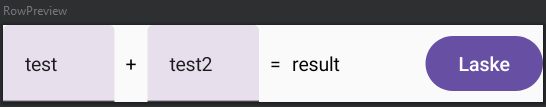
\includegraphics[width=0.8\textwidth]{figures/exercise-5-row-preview.png}
    \caption{Yhden laskurin rivin esikatselu}
    \label{fig:exercise-5-row-preview}
\end{figure}

Kun laskuoperaation merkki annetaan Composablelle parametrina, on koko laskimen
muodostaminen hyvin suoraviivaista UIn puolesta, kuten koodista
\ref{lst:full-calculator} ja kuvasta \ref{fig:exercise-5-calculator-preview}
nähdään.

\begin{lstlisting}[
    basicstyle=\small,
    label={lst:full-calculator},
    caption={CalculatorScreen-koodin hahmottelua},
    language=Kotlin,
]
@Composable
fun CalculatorScreen(
    modifier: Modifier = Modifier,
) {
    Column(modifier = modifier) {
        CalculatorRow(operator = "+")
        CalculatorRow(operator = "-")
        CalculatorRow(operator = "x")
        CalculatorRow(operator = "/")
    }
}
\end{lstlisting}

\begin{figure}[h!]
    \centering
    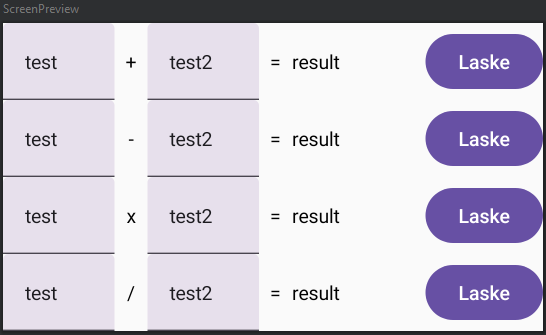
\includegraphics[width=0.8\textwidth]{figures/exercise-5-calculator-preview.png}
    \caption{Oheisen CalculatorScreen-koodin tuottama esikatselu}
    \label{fig:exercise-5-calculator-preview}
\end{figure}

Sovellukseen haluttiin toinen näkymä. Yksinkertaisuuden vuoksi lisätään näkymään
vain normaali painike ja painikkeen alle lista tehdyistä laskutehtävistä. Näkymä
saadaan nopeasti hahmoteltua ja esikatselua kuvassa
\ref{fig:exercise-5-history-preview} näkyvästä esikatselusta

\begin{figure}[h!]
    \centering
    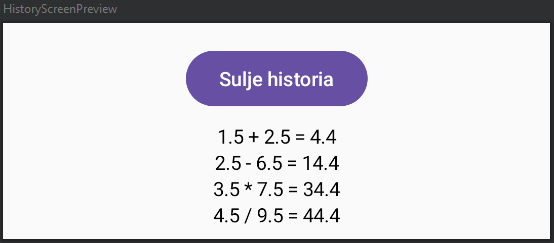
\includegraphics[width=0.8\textwidth]{figures/exercise-5-history-preview.png}
    \caption{Historianäkymän esikatselu}
    \label{fig:exercise-5-history-preview}
\end{figure}

Näkymien oltua karkeasti valmiina, on aika toteuttaa varsinainen
toiminnallisuus. Laskutoiminnallisuus saadaan yksinkertaisesti lisäämällä
riveille parametriksi funktio, joka hoitaa laskemisen. Tämän jälkeen riville
pitää vain toteuttaa Laske-painikkeelle käsittelijä, joka parsii rivillä
olevien kenttien numerot ja välittää ne parametrina saadulle lasku funktiolle,
jos numerot ovat kelvollisia. Mikäli numeron parsiminen ei onnistu tai lasku
funktio palauttaa null:in (vain jos yritetää jakaa nollalla), näytetään
käyttäjälle "ERROR"-teksti tuloksen sijaan. Jos puolestaan edes toinen kentistä
on tyhjä niin tyhjennetään tulosteksti.

Numeroiden parsiminen on sinääli haastava tehdä ilman ongelmia jo mm. eri
välimerkkien takia. Tämän huomaa hyvin kun saa sovelluksen kaatumaan useamman
kerran kun käyttää pilkkua pisteen sijaan. Try-catch parsimisen ja laskennan
ympärille ja käyttäjälle näkyviin "ERROR" muissakin virhetilanteissa niin
estetään sovelluksen kaatuminen. Mahdollisesti käyttämällä NumberFormat tms.
luokkaa voitaisiin parsiminen hoitaa perustuen Localeen, jolloin pilkut
voisivat toimia pisteen sijaan, mutta jotta asia pidetään yksinkertaisena,
käytetään vain valmista toDoubleOrNull-funktiota.

Seuraavaksi olisi laskujen tallentamisen vuoro ja ohjeessa sanotaan, että se
voidaan toteuttaa tavallisena tiedostoon kirjoituksena eikä tietokantaa
kannattaisi tähän rakentaa. Jääräpäänä en suostu tietoja tallentamaan
tiedostoon ellei ole ihan välttämätöntä kun liian monta kertaa törmännyt
projektiin, jossa on todettu ettei tietokantaa tarvitsisi vaikka oikeasti
tarvitsee ja joutunut näkemään ylimääräistä vaivaa sen vuoksi. Toki näin
harjoitustehtävässä, johon kukaan ei tule enää ikinä koskemaan, ei kyseistä
tilannetta tule tapahtumaan. Kuitenkin tehtävän annoin muotoilu antaa ymmärtää,
ettei tietokantaa tulisi käyttää sen aiheuttaman ylimääräisen vaivan vuoksi,
eikä niinkään sen vuoksi, että opettelisi kirjoittamaan tiedostoihin. Siispä
pitääkseni harjoituksen yksinkertaisena, käytän tietokantaa sen ollessa
huomattavasti nopeampaa ja yksinkertaisempaa toteuttaa kuin lähteä tutkimaan
miten tiedostoihin kirjoittaminen/lukeminen tapahtuu.

Tietokannan määrittämisessä toki onnistui pari huolimattomuutta tapahtumaan,
jonka seurauksena törmäsi käännösvirheeseen, joka johtui puuttuvasti
riippuvuudesta. Tämän lisäksi unohtui määrittää ID generoitumaan
automaattisesti, joten käytössä olleella IGNORE-käytönnöllä seurasi se, että
vain ensimmäinen tallentui tietokantaan. Kannan rakenteen muuttamisen jälkeen
sovellus kaatui vielä kerran kun unohtui muuttaa kannan versiota. Ilmeentyneet
ongelmat pieniä ja korjaantuivat kaikki helposti virheen perusteella ilman
tarkempaa tutkimista.

Hiukan UI:n tyylien säätämisen jälkeen sovellus onkin valmis käytettäväksi.
Käytettävyyttä saadaan parannettua, kun aktivoidaan numeronäppäimistö kenttiin
normaalin näppäimistön sijaan. Lisäksi historia näkymään lisätään scrollattava
lista, joka tukee suuria määriä tuloksia (LazyColumn). Vaihdetaan myös tehtyjen
laskujen järjestys käänteiseksi eli uusin ylimmäiseksi. Lopullisen sovelluksen
näkee kuvista \ref{fig:exercise-5-final-1} ja \ref{fig:exercise-5-final-2}.

\begin{figure}[h!]
\centering
\begin{minipage}[b]{.4\textwidth}
    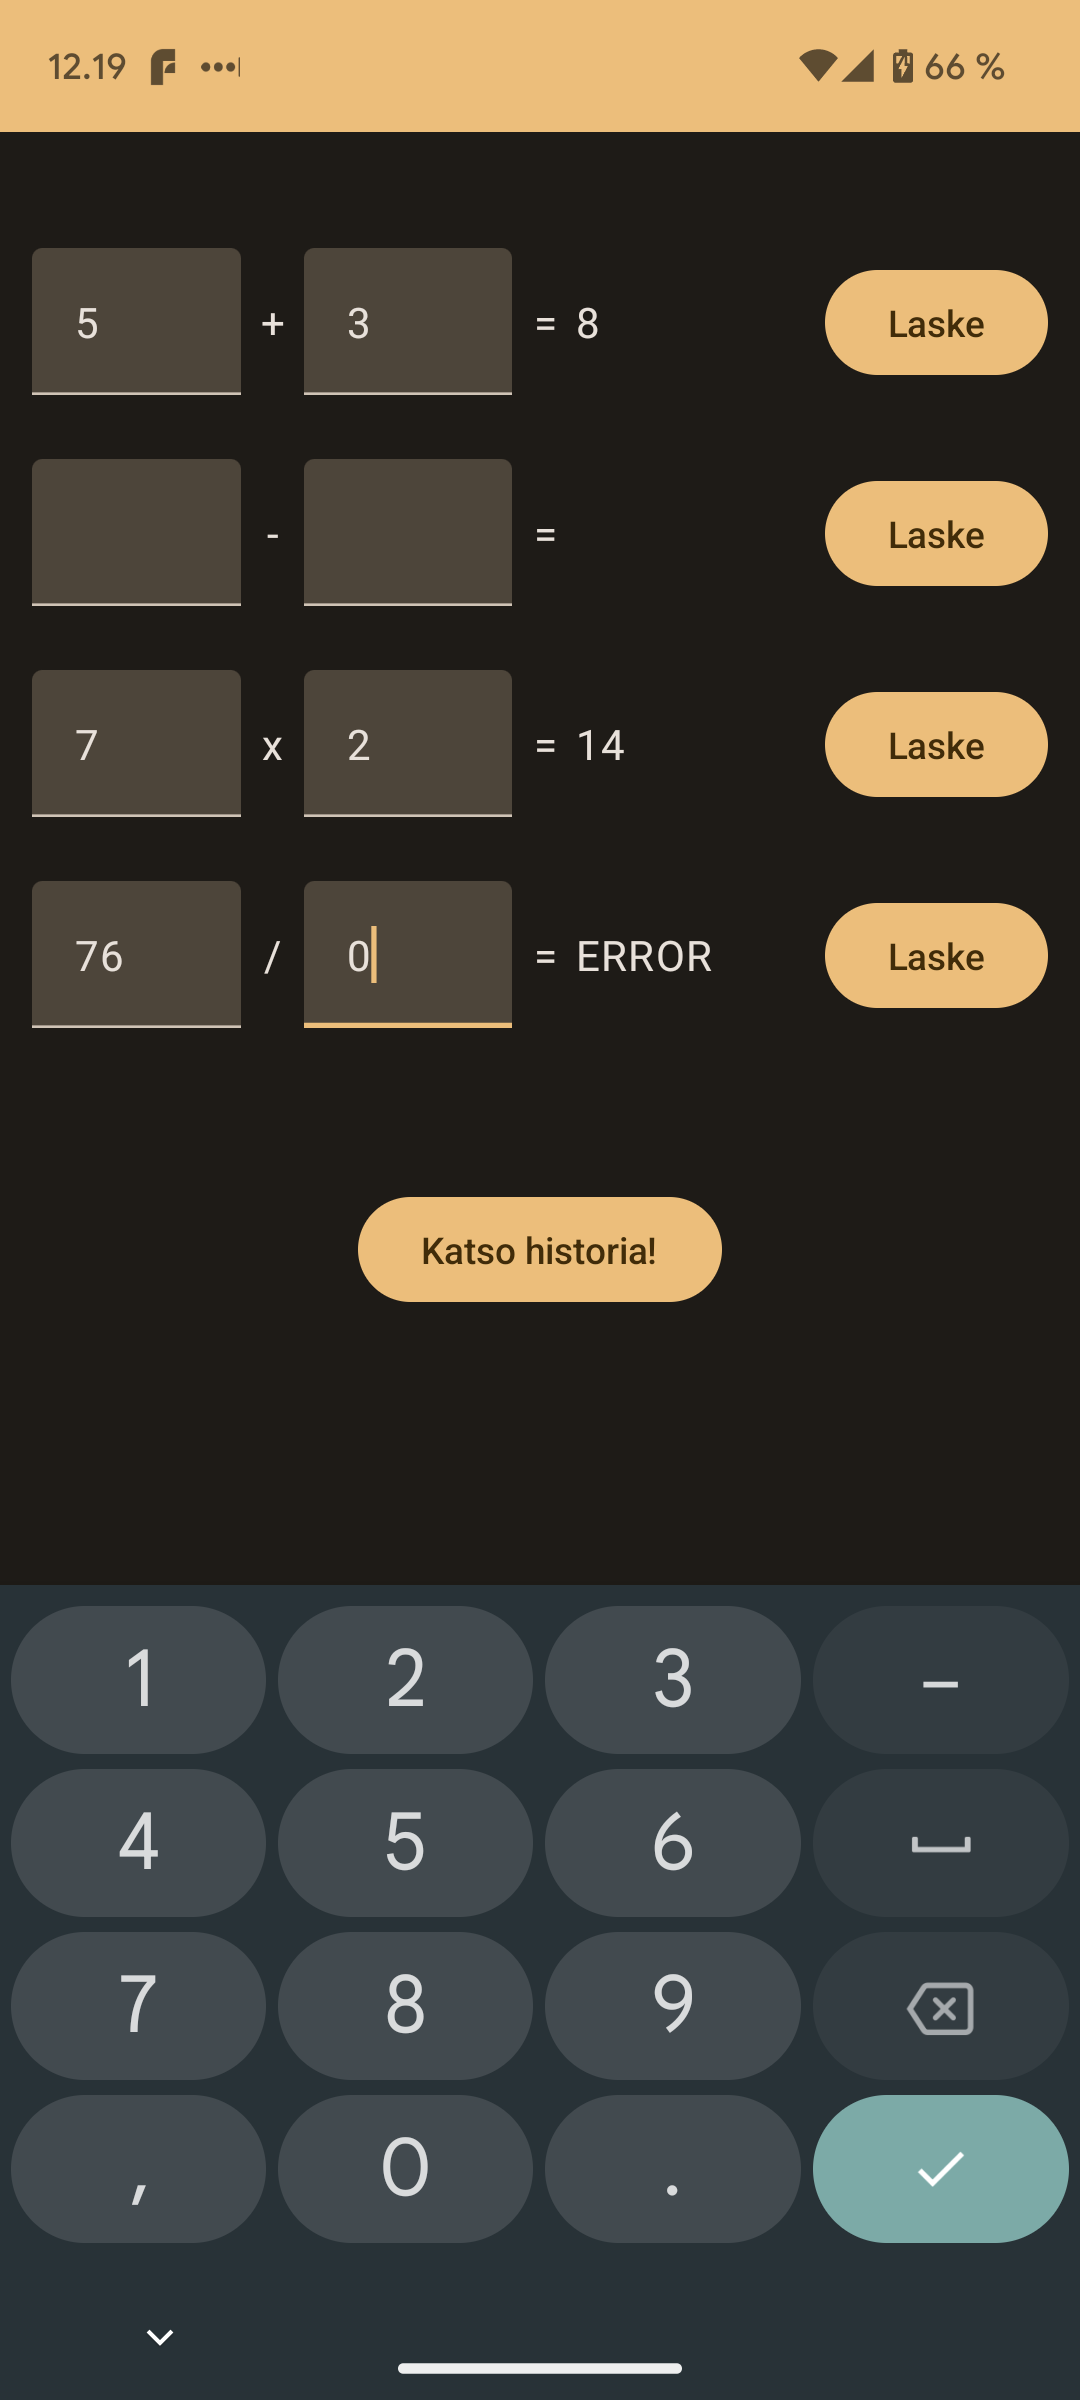
\includegraphics[width=\textwidth]{figures/exercise-5-final-1.png}
    \caption{Laskin näkymä}
    \label{fig:exercise-5-final-1}
\end{minipage}\qquad
\begin{minipage}[b]{.4\textwidth}
    
\includegraphics[width=\textwidth]{figures/exercise-5-final-2.png}
    \caption{Historia näkymä}
    \label{fig:exercise-5-final-2}
\end{minipage}
\end{figure}

Parannettavaa löytyy toki yhä tähänkin, mm. voisi käyttää repositoryja eikä
suoraan kutsua dao:a. Saavutettavuus kaipaisi tässäkin parantamista kuten myös
testejä. Nämä kaksi puutetta tulevat tosin todennäköisesti jatkuvaan jokaisen
harjoitustehtävän kohdalla.

Tämän harjoituksen tekemiseen tuli katseltua esimerkkiä Googlen kurssin
harjoitustehtävistä Inventory App \parencite{GithubGoogleDevTrainingInventory},
Bus Schedule \parencite{GithubGoogleDevTrainingBusSchedule}, Cupcake
\parencite{GithubGoogleDevTrainingCupcake} ja Unscramble
\parencite{GithubGoogleDevTrainingUnscramble}.

\section{Harjoitus 6}

Harjoituksen aiheeksi valittu paikan tallentaminen. Tietokantaan määritelty
neljä kenttää yksilöivän tunnisteen lisäksi kuten koodista
\ref{lst:location-data-class} on nähtävissä.

\begin{lstlisting}[
    basicstyle=\small,
    label={lst:location-data-class},
    caption={Location data class},
    language=Kotlin,
]
@Entity(tableName = "location")
data class Location(
    @PrimaryKey(autoGenerate = true)
    val id: Long = 0,

    val longitude: Double,
    val latitude: Double,
    val timestamp: Long,
    val notes: String,
)
\end{lstlisting}

Koska harjoituksessa painotuksena nimenomaan tietokanta ja sinne tiedon
tallentaminen, toteutan ensin tietokanta puolen ja vasta sen jälkeen lähden
hahmottelemenaan käyttöliittymää. Koska tietokanta tuli toteutettua jo
edellisessä harjoituksessa, menee sen toteuttaminen hyvinkin suoraviivaisesti.
Kuitenkin vastaan tulee aluksi ongelma, ettei Room tue OffsetDateTime-tyyppiä,
joten joko pitäisi rakentaa convertteri muuttamaan se sopivampaan muotoon tai
tyytyä siihen, että tallennetaan ajanhetki UNIX-aikana, poikkeuksena kuitenkin,
että käytetään millisekunteja sekuntien sijaan.

Tämän jälkeen listanäkymän hahmoittelu tiedoille, kuten esikatselussa
\ref{fig:exercise-6-location-screen} näkyy. Pari material iconia tietojen
kanssa niin ulkoasu näyttää merkittävästi paremmalta vaikka onkin hyvin
pelkistetty ilman tyylittelyä.

\begin{figure}[h!]
    \centering
    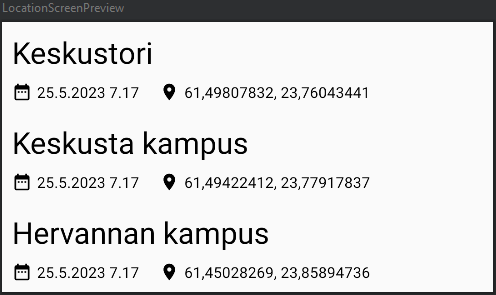
\includegraphics[width=0.8\textwidth]{figures/exercise-6-location-screen.png}
    \caption{Sijaintien listanäkymän esikatselu}
    \label{fig:exercise-6-location-screen}
\end{figure}

Haluan erotella tietojen lisäämisen perusnäkymästä, mutta täysin oman näkymän
tekeminen tuntuu myös vähän "tylsältä" ratkaisulta. Mahdollisesti dialogi tms.
voisi olla sellainen minkä haluaisin. Pienen Googlailun jälkeen mitä eri
komponentteja on saatavilla, törmään Material Designissa oleviin Bottom
Sheetseihin \parencite{MaterialComponentsBottomSheets}, jotka vaikuttavat
siistiltä ratkaisulta, vaikka niiden tarkoitus onkin ilmeisesti olla hiukan
enemmän lisätoiminnoille ja -sisällölle kuin niinkään uuden asian lisäämiseksi.
En ole kuitenkaan koskaan noita käyttänyt, joten aika kokeilla. Nopeahko
kuvan \ref{fig:exercise-6-location-insert-screen} mukainen hahmotelma
käyttöliittymälle, jonka jälkeen aika luoda ViewModelit ja yhdistää niiden
avulla data ja käyttöliittymä.

\begin{figure}[!ht]
    \centering
    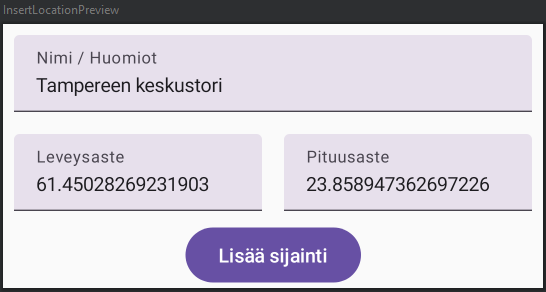
\includegraphics[width=0.8\textwidth]{figures/exercise-6-location-insert-screen.png}
    \caption{Sijaintien lisäys lomakkeen esikatselu}
    \label{fig:exercise-6-location-insert-screen}
\end{figure}

\begin{wrapfigure}{r}{0.3\textwidth}
    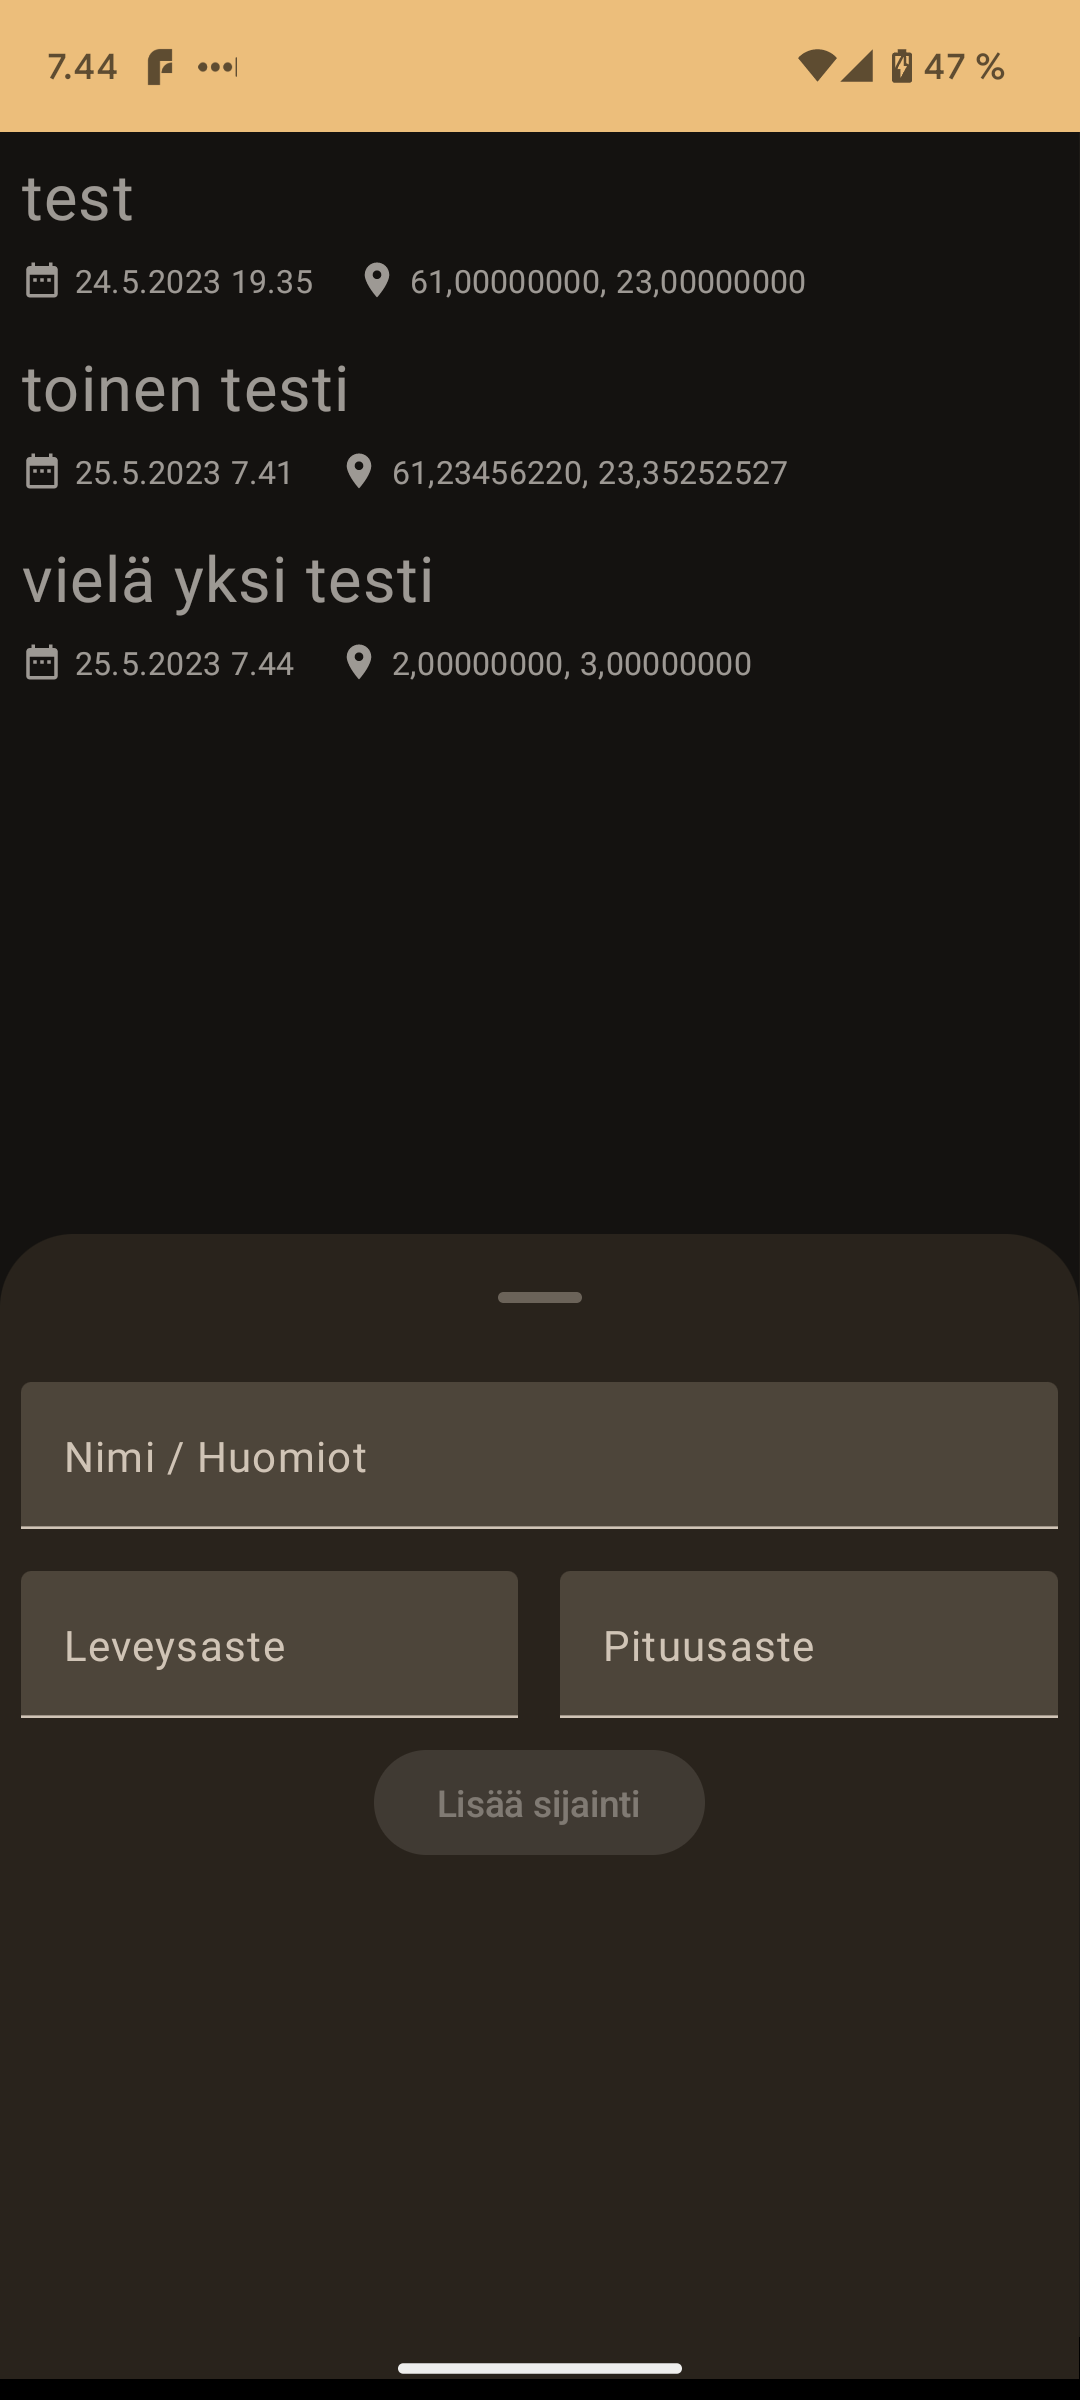
\includegraphics[width=0.3\textwidth]{figures/exercise-6-final.png}
    \caption{Kuvankaappaus lopullisesta sovelluksesta puhelimessa}
    \label{fig:exercise-6-final}
\end{wrapfigure}

Hiukan testailua puhelimella niin huomaa kaksi käytettävyyteen parannettavaa
asiaa: tekstikenttiihin hyvä lisätä labelit, jotka näkyvätkin jo kuvassa
\ref{fig:exercise-6-location-insert-screen}. Lisäksi tiedon lisäämisen jälkeen
käyttäjälle mukavampaa, jos vanhat tiedot tyhjennetty kentistä ettei uuden
tiedon lisäämisessä tarvitse aloittaa kenttien tyhjentämisellä. Muutaman
sijainnin lisäämisen jälkeen saadaan kuvankaappaus \ref{fig:exercise-6-final}
tämän harjoiuksen lopullisesta sovelluksesta.

\section{Harjoitus 7}

Tämä harjoitus on jatkoa edelliselle harjoitukselle, joten muutokset tehdään
versionhallintaakin harjoitustehtavat/harjoitus6/ -kansioon. Mikäli haluaa
tarkistella harjoitus 6 jälkeistä tilannetta, onnistuu se helposti Gitlabin
web-käyttöliittymässä vaihtamalla main-branchi tagiin ''exercise-06'' kuvan
\ref{fig:gitlab-change-branch-to-tag}. Vaihtoehtoisesti toki perus checkout
kyseiseen tagiin toimii, jos tarkastelee koodia omalta koneelta. Vastaavat
tagit tarkoitus tehdä muillekkin, jotka jatkavat edellistä harjoitusta.

\begin{figure}[!ht]
    \centering
    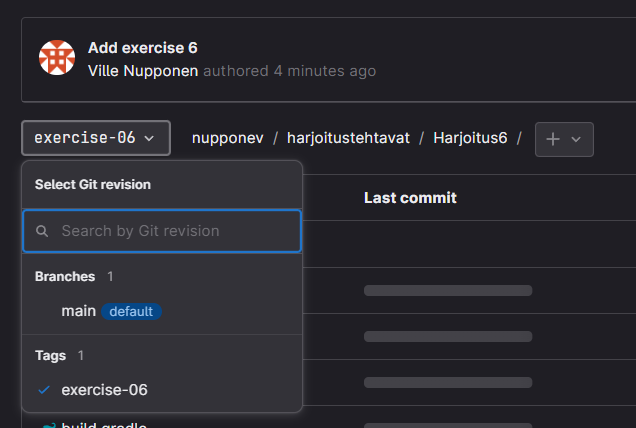
\includegraphics[width=0.8\textwidth]{figures/gitlab-change-branch-to-tag.png}
    \caption{Gitlabissa koodin näyttäminen tietyn tagin mukaan}
    \label{fig:gitlab-change-branch-to-tag}
\end{figure}

Harjoitus 7 olettaa ilmeisesti, että edellisellä harjoituksessa ei olisi
käytetty Composea vaan tehty perinteisillä View komponenteilla. Lähin vastine
Composen kanssa lienee se, että teen oman Composablen. Lisäksi harjoituksessa
ohjeistettu käyttämään RecyclerView-ominaisuutta, jolle hyvä vastine Composen
puolella on LazyColumn, joka oli jo käytössä.

Varsinaisen koodin muuttamiseen ei mene minuuttia kauempaa, mutta ilmeisesti
nyt tuli vastaan mahdollisesti ensimmäinen ongelma bind mountin kanssa. Eri
tiedostojärjestelmät ilmeisesti huomioivat kirjainkoon erilailla. Tämän
seurauksena onnistuin lisäämään harjoitus6:n versionhallintaan kahdesti. Toinen
kansio alkoi isolla kirjaimella ja toinen pienellä. Muutokset olin tietysti
ehtinyt jo pushata ja suoraan main-branchiin, joten historian korjaus ei
onnistu branchin suojauksen vuoksi. Uutta committia siis perään, jossa
poistettu duplikaatti. Asiaa toki hiukan hankaloitti se ettei tiedostoissa ne
näkynyt kahtena vaan ainoastaan git tunnisti ne erillisiksi. Sen tarkmmin
perehtymättä ongelma korjattu, muutokset tehty uudelleen ja testattu.

\section{Harjoitus 8}

Tässä harjoituksessa lisätään mahdollisuus järjestää sijainnin aikaleiman
mukaan, joko laskevaan tai nousevaan järjestykseen. Järjestys tallennetaan,
jotta järjestys on seuraavalla sovelluksen käyttökerralla sama eikä nollaannu
joka kerta kun sovelluksen avaa uudelleen. Toteutetaan lisäksi mahdollisuus
poistaa tallennettuja sijainteja.

Käyttäjän preferenceistä saadaan tehtyä käytevästi oma repository, ja sen myötä
ketjujettua Flow peräkkäin. Toki tässä tapauksessa halutaan saada myös
ensimmäinen tieto UiState:lle, joten sisäkkäin laittaminen auttaa siinä, kuten
koodissa \ref{lst:nested-flows} on tehty. Esimerkkejä ketjutuksee ja sisäkkäin
laittamiseen on saatu blogipostista \parencite{KotlinFlowNestingVSChaining}.

\begin{lstlisting}[
    basicstyle=\small,
    label={lst:nested-flows},
    caption={Useamman flown käyttäminen yhdessä},
    language=Kotlin,
]
@OptIn(FlowPreview::class)
val locationUiState: StateFlow<LocationUiState> =
    userPreferencesRepository.isAscOrder
        .flatMapMerge { isAscOrder ->
            (if (isAscOrder) locationRepository.getAllOrderByTimestampAsc()
            else locationRepository.getAllOrderByTimestampDesc())
                .map { locations ->
                    LocationUiState(locations = locations, isAscOrder = true)
                }
        }
        .stateIn(
            scope = viewModelScope,
            started = SharingStarted.WhileSubscribed(TIMEOUT_MILLIS),
            initialValue = LocationUiState()
        )
\end{lstlisting}

Jotta UI saadaan hiukan ''eloisammaksi'' niin laitetaan järjestyksen
vaihtopainikkeeseen hiukan animointia niin pääsee niitäkin testaamaan tässä
samalla. Animaatioiden tekemisen tueksi löytyi hyvä blogi postaus
\parencite{CardFlipAnimationWithJetpackCompose}.

Emulattorista löytyy kätevä screen recorder, jolla saadaan nauhoitettua
animaatiota. Videon laittaminen kuitenkin tähän dokumenttiin on jokseenkin
haastavaa, joten on se saatavilla Oppimispäiväkirja repositoryssa other
-kansiossa.

Merkittäviä ongelmia järjestämisessä ei tule, kunhan animaatioon laittaa oikean
luvun eikä vahingossa kymmenkertaista (nollan 180f vs 1800f) niin ei iconi
kierry liian montaa kertaa X-akselin ympäri. Lisäksi hyvä olla tarkkana
kopioinnissa ettei jätä molempiin tietokantakyseyihin järjestykseksi DESC, kun
silloin ei oikein järjestys vaihdu vaikka painike toimiikin.

Poistaminen voitaisiin toteuttaa usealla eritavalla, mutta yksinkertaisuuden ja
jonkun uuden asian oppimiseksi, valitsin tavaksi kuunnella "pitkää painallusta"
ja avata sen myötä dialogin, joka kysyy poistetaanko vai ei. Tähän tueksi
löytyi yksinkertainen ja selvä postaus \parencite{DevelopersMemoLongPress}.

Vaikutteita tähän ja jonkin verran myös harjoituksiin 6 ja 7 se on tullut
''Now In Android''-esimerkistä \parencite{GithubAndroidNowInAndroid}. Lisäksi
Prefence DataStoren käyttämiseen käytetty tukena ''Dessert Release App''
-harjoitusta \parencite{GithubGoogleDevTrainingDessertRelease}.

\section{Harjoitus 11}

Harjoituksessa tavoitteena on saada näkyviin puhelimen asentoon liittyvät
arvot. Olen kuitenkin vuosia sitten noiden kanssa testaillut, joten
mielenkiinnon vuoksi otettu harjoituksessa mainittu vapaaehtoinen optio, jossa
haetaan useampien sensoreiden arvot. Koska kiinnostus tietää mitä kaikkea
mahdollista saada, haetaan kaikki saatavilla olevat sensorit ja niiden arvot.

Jottei turhaan kuormiteta puhelinta kaikilla sensoreiden datalla sovelluksen
ollessa päällä, toteutetaan yksinkertainen lista SensorManagerin antamista
sensoreista kuten kuvasta \ref{fig:exercise-11-sensor-list} nähdään. Painamalla
haluttua sensoria, saadaan rekisteröityä sensorin kuunteleminen ja näytetty
saatu data kuvan \ref{fig:exercise-11-sensors-selected} mukaisesti.

\begin{figure}[h!]
    \centering
    \begin{minipage}[b]{.4\textwidth}
        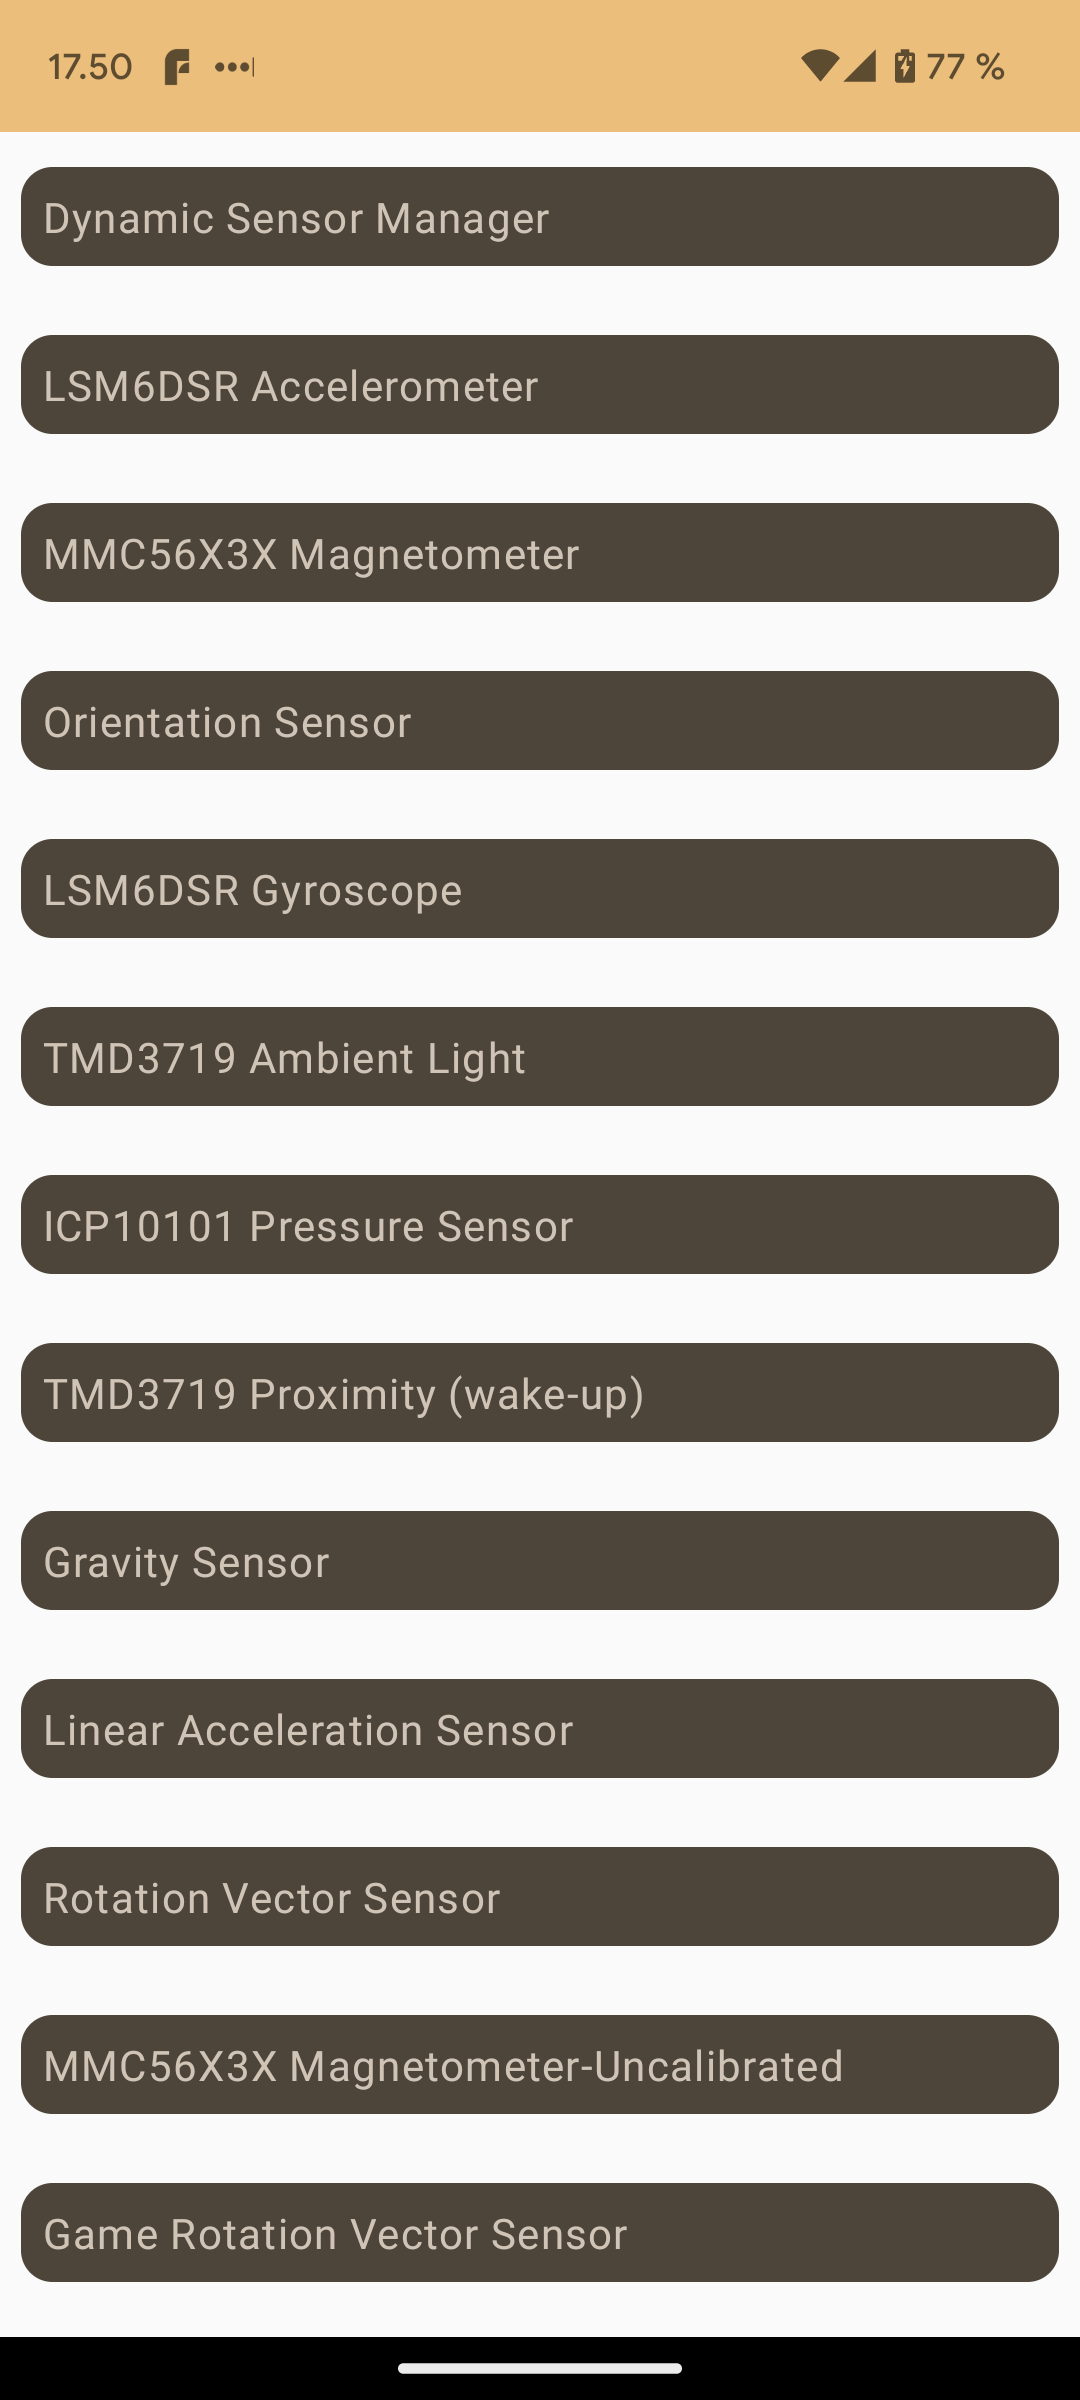
\includegraphics[width=\textwidth]{figures/exercise-11-sensor-list.png}
        \caption{Lista kaikista saatavilla olevista sensoreista}
        \label{fig:exercise-11-sensor-list}
    \end{minipage}\qquad
    \begin{minipage}[b]{.4\textwidth}
        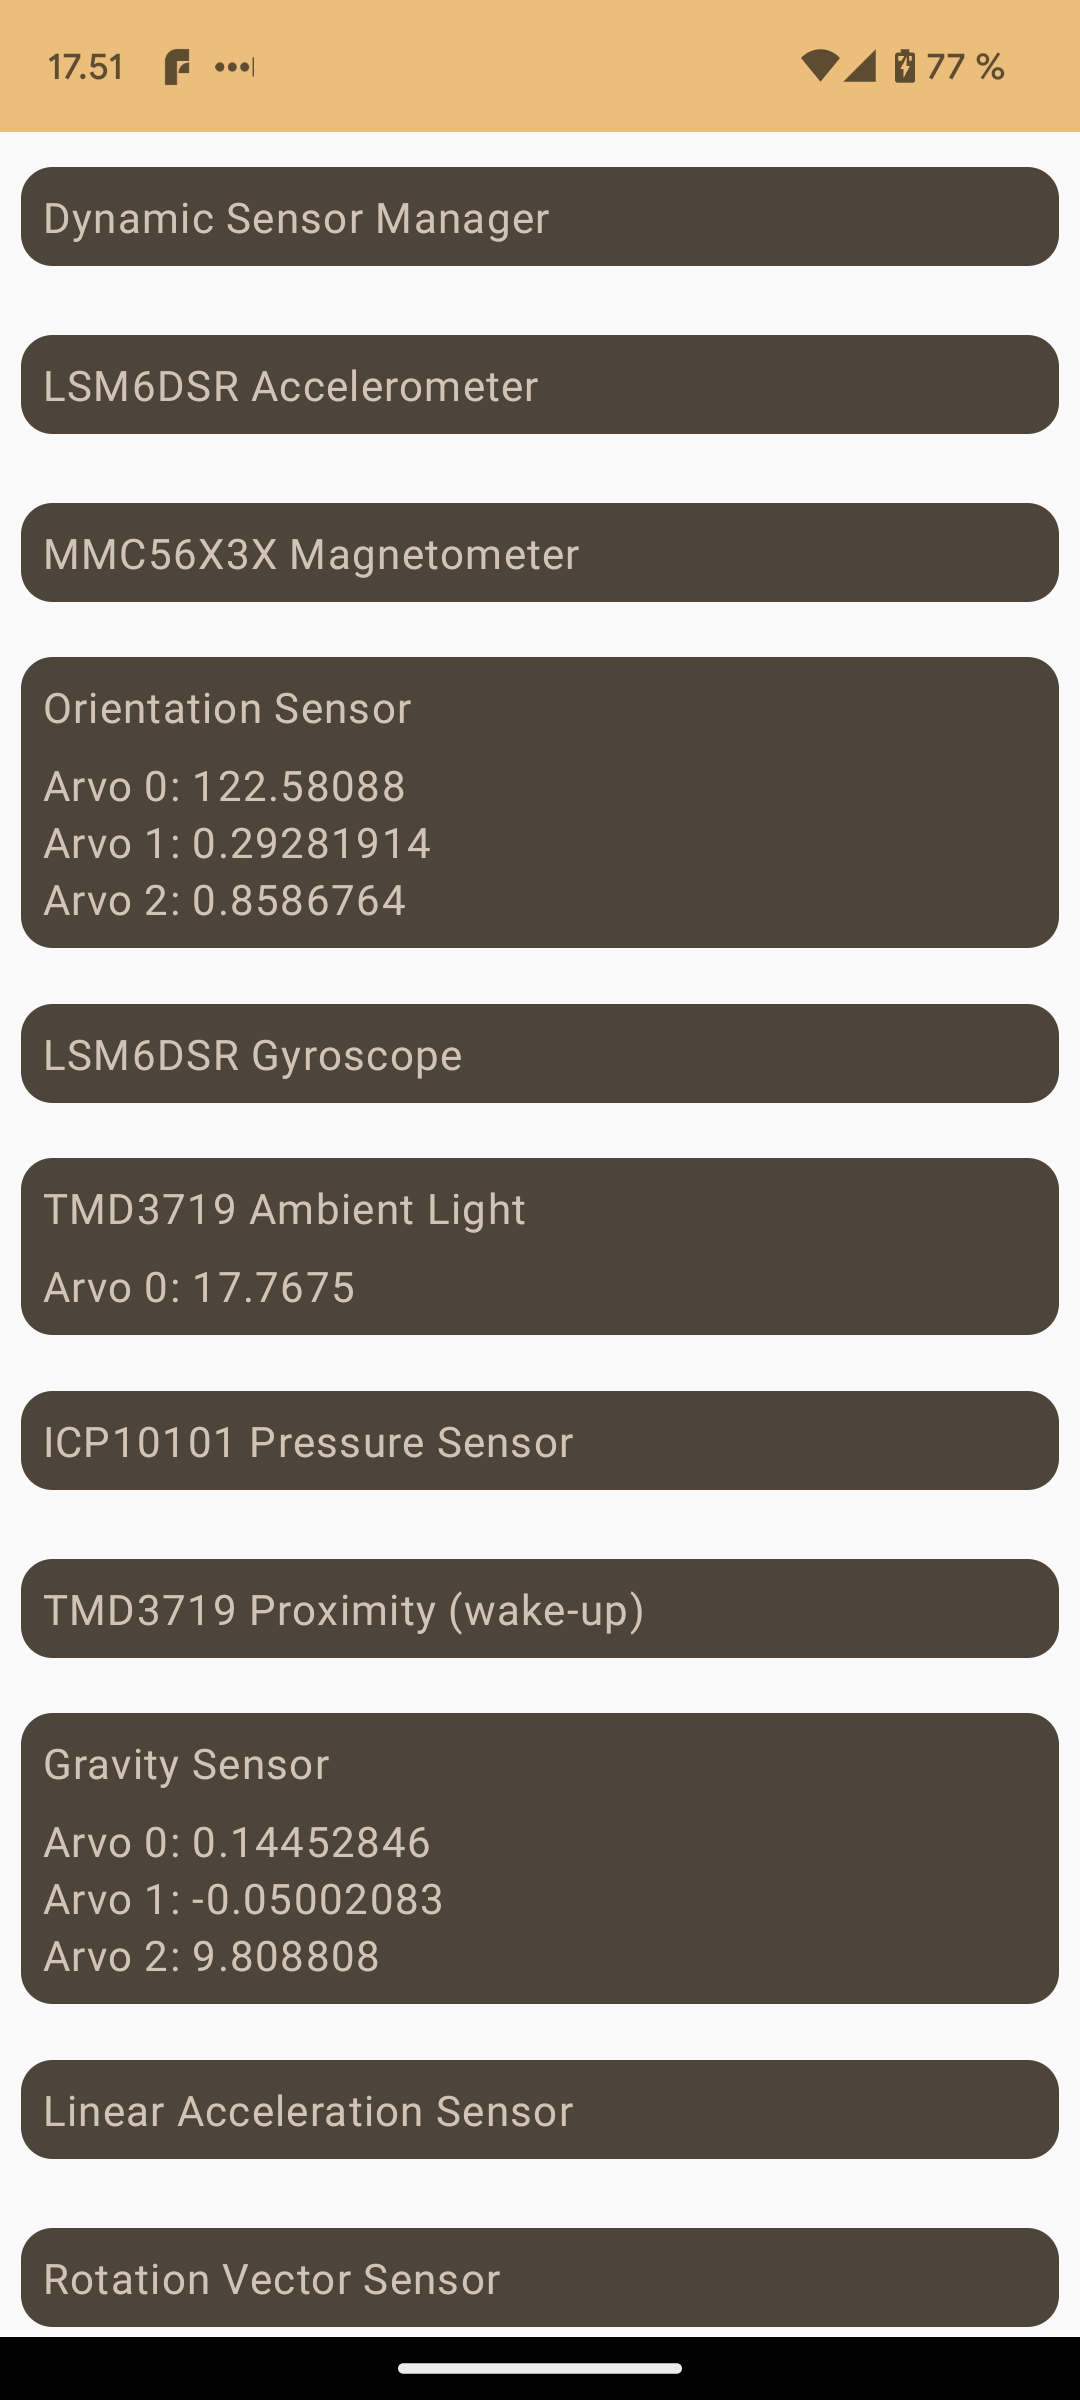
\includegraphics[width=\textwidth]{figures/exercise-11-sensors-selected.png}
        \caption{Sensori lista, jossa valittu muutama sensori}
        \label{fig:exercise-11-sensors-selected}
    \end{minipage}
\end{figure}

Sensorien ja sensorien datan näyttäminen on melko suoraviivaista.
Harjoituksessa tallennettiin lista sensoreista UIStateen ja erillinen lista
sensorien antamille tapahtumille. Koska UI:ssa näytetään vain uusin tapahtuma,
riittää yhden tapahtuman tallentaminen yhtä sensoria kohden. Tällöin tähän
toimii kätevästi Map, jolle saadaan annettua avaimeksi sensoria vastaava
uniikki avain ja arvoksi sensorin antamat arvot. UI ei kuitenkaan päivitä
arvoja, vaikke ne Map:ssa muuttuvatkin. Tämä johtunee siitä, että tehdään
tarkistus, onko tiedot samat ja kyseinen tarkistus ei tarkista kaikkia arvoja
vaan käyttää UiStaten oletus equals/hashCode, jotka tarkistavat ilmeisesti
oletuksena vain onko viittaus samoihin olioihin eikä olioiden sisällä olevien
arvojen muuttumisia. Ylikirjoittamalla kyseiset funktiot, saadaan arvot
muuttumaan UI.ssa.

Harjoitusta varten tehtävänannossa linkatut oheismateriaalit
\parencite{AndroidDevelopersDocsSensors}
\parencite{AndroidDevelopersCodelabsSensorData} kattoivat erittäin hyvin kaiken
harjoitukseen tarvittavan tiedon.

Voisi olla hyödyllistä käyttää DisposableEffect:ia apuna siihen, että sensorien
datan seuranta lopetetaan kun sensorin dataa ei enää näytetä. Sovelluksessa ei
kuitenkaan ole mitään muita näkymiä yms., joten tässä tapauksessa ei niin
oleellinen, vaikka datan näyttäminen onkin turhaa niiden sensorien osalta,
jotka eivät näy listan ollessa liian pitkä / scrollattu eri kohtaan.

\section{Tuntikirjanpito}

Oheiseen talukkoon on koottu harjoitustehtäviin käytetyt tunnit.

\begin{table}[H]
  \centering
  \label{tab:other-studing-working-hours}
  \begin{tabular*}{\linewidth}{@{\extracolsep{\fill}} l c c c r }
    \textbf{Tekeminen} & \textbf{Päivämäärä} & \textbf{Aloitettu} & \textbf{Lopetettu} & \textbf{Määrä} \\
    \hline
    Harjoitus 2  & 23.05.2023 & 05:15 & 05:25 &    10m \\
    Harjoitus 3  & 23.05.2023 & 05:25 & 08:05 & 2h 40m \\
    Harjoitus 3  & 24.05.2023 & 06:15 & 06:30 &    15m \\
    Harjoitus 4  & 24.05.2023 & 06:30 & 08:40 & 2h 10m \\
    Harjoitus 5  & 24.05.2023 & 08:50 & 09:05 &    15m \\
    Harjoitus 5  & 24.05.2023 & 09:25 & 12:55 & 3h 30m \\
    Harjoitus 6  & 24.05.2023 & 16:30 & 19:40 & 3h 10m \\
    Harjoitus 6  & 25.05.2023 & 06:40 & 08:30 & 1h 50m \\
    Harjoitus 7  & 25.05.2023 & 08:30 & 09:10 &    40m \\
    Harjoitus 8  & 25.05.2023 & 12:35 & 15:30 & 2h 55m \\
    Harjoitus 8  & 26.05.2023 & 08:30 & 08:45 &    15m \\
    Harjoitus 11 & 26.05.2023 & 09:00 & 10:00 & 1h 00m \\
    Harjoitus 11 & 26.05.2023 & 10:50 & 12:50 & 2h 00m \\
    Harjoitus 11 & 12.07.2023 & 17:00 & 18:30 & 1h 30m \\
    Harjoitus  8 & 12.07.2023 & 18:50 & 19:50 & 1h 00m \\
    Harjoitus  8 & 14.07.2023 & 12:35 & 12:45 &    10m \\
    \hline
    \multicolumn{4}{l}{\textbf{Yhteensä}} & \textbf{23h 30m} \\
  \end{tabular*}
\end{table}
